% ================================================================
% The Retrieve and Connect version of latex/starters/targeted/KS3/numberSense/numberSenseStarters_workedSolutions.tex
%
% This is the same deck as the one above, made by renaming the titles in it.
% Every slide that was a numbered starter is now titled
% "Retrieve and Connect", and the word is renamed wherever else a title
% used it. Nothing outside a title has been changed.
%
%   made from           latex/starters/targeted/KS3/numberSense/numberSenseStarters_workedSolutions.tex
%   retitling rules     version 1
%
% Please don't edit this file. It is written again from the one it was
% made from whenever that changes, so an edit here would be lost - edit
% that file instead and this one follows.
% ================================================================
% Root file used ashow macros
\documentclass{beamer}
\usepackage{tikz}
\usetikzlibrary{calc}
\usepackage{xcolor}
\usepackage{multicol}
\usepackage{amsmath}
\usepackage{amssymb}

% ================================================================
% Answer-overlay helpers
% ================================================================
\newcommand{\ablank}[1]{%
  \alt<2>{\textcolor{red}{#1}}{\underline{\phantom{#1}}}%
}
\newcommand{\ashow}[1]{\uncover<2->{\textcolor{red}{\small #1}}}
\newcommand{\ashowq}[1]{\alt<2->{\textcolor{red}{\small #1}}{?}}

% Answers drawn straight on to a TikZ diagram, revealed on overlay 2 like \ashow.
% Space is reserved on overlay 1, so the diagram does not move between slides.
\usetikzlibrary{overlay-beamer-styles}
\tikzset{
  ans/.style     = {red, thick, visible on=<2->},
  ansfill/.style = {red!15, visible on=<2->},
  anslab/.style  = {red, font=\tiny, visible on=<2->},
}

% Used by the worked solutions rather than by this deck, so that each worked
% solution is first a question with room to write in and then the answer.
\newlength{\aworkpad}
\setlength{\aworkpad}{8mm}
\newcommand{\awork}[1]{%
  \par\vspace{\aworkpad}%
  \uncover<2->{#1}%
  \par\vspace{\aworkpad}%
}

% Tighter list spacing, so eight questions fit on one frame.
\newcommand{\qtight}{%
  \setlength{\itemsep}{0pt}\setlength{\parskip}{0pt}\setlength{\parsep}{0pt}%
  \setlength{\topsep}{0pt}\setlength{\partopsep}{0pt}%
}
\setlength{\columnsep}{8pt}

\title{Number Sense: Retrieve and Connects}
\author{}
\date{}

\begin{document}

\frame{\titlepage}

\begin{frame}{Contents}
\small
\begin{columns}[T]
\column{0.5\textwidth}
\textbf{Questions and short answers}
\begin{itemize}
\item \hyperlink{q-st1}{\beamergotobutton{Retrieve and Connect 1}}
\item \hyperlink{q-st2}{\beamergotobutton{Retrieve and Connect 2}}
\item \hyperlink{q-st3}{\beamergotobutton{Retrieve and Connect 3}}
\item \hyperlink{q-st4}{\beamergotobutton{Retrieve and Connect 4}}
\item \hyperlink{q-st5}{\beamergotobutton{Retrieve and Connect 5}}
\end{itemize}
\column{0.5\textwidth}
\textbf{Worked solutions}
\begin{itemize}
\item \hyperlink{work-st1}{\beamergotobutton{Retrieve and Connect 1}}
\item \hyperlink{work-st2}{\beamergotobutton{Retrieve and Connect 2}}
\item \hyperlink{work-st3}{\beamergotobutton{Retrieve and Connect 3}}
\item \hyperlink{work-st4}{\beamergotobutton{Retrieve and Connect 4}}
\item \hyperlink{work-st5}{\beamergotobutton{Retrieve and Connect 5}}
\end{itemize}
\end{columns}
\end{frame}

%------------------------------------------------
% STARTER 1: Number Lines and Place Value
%------------------------------------------------
\begin{frame}{Retrieve and Connect}
\hypertarget{q-st1}{}

\vspace{-2.5em}

\begin{columns}[T]

\column{0.30\textwidth}
\begin{center}
\vspace{3em}
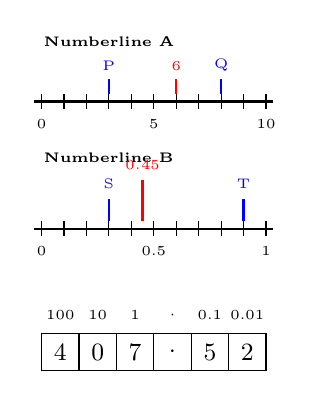
\begin{tikzpicture}[scale=0.95]

% --- Line A: 0 to 10, ticks every 1 ---
\node[font=\tiny\bfseries, anchor=west] at (-0.1,4.6) {Numberline A};
\draw[thick] (-0.1,3.8) -- (3.1,3.8);
\foreach \x in {0,0.3,0.6,0.9,1.2,1.5,1.8,2.1,2.4,2.7,3}
  \draw (\x,3.7) -- (\x,3.9);
\foreach \x/\lab in {0/0,1.5/5,3/10} \node[font=\tiny] at (\x,3.5) {\lab};
% Given points: P at 3, Q at 8. Kept low, so they stay clear of the Line A heading.
\draw[blue, thick] (0.9,3.9) -- (0.9,4.1);
\node[blue, font=\tiny] at (0.9,4.28) {P};
\draw[blue, thick] (2.4,3.9) -- (2.4,4.1);
\node[blue, font=\tiny] at (2.4,4.28) {Q};
% --- Q3 answer: 6 marked on Line A ---
\draw[ans] (1.8,3.9) -- (1.8,4.1);
\node[anslab] at (1.8,4.28) {$6$};

% --- Numberline B: 0 to 1 in tenths ---
\node[font=\tiny\bfseries, anchor=west] at (-0.1,3.05) {Numberline B};
\draw[thick] (-0.1,2.1) -- (3.1,2.1);
\foreach \x in {0,0.3,0.6,0.9,1.2,1.5,1.8,2.1,2.4,2.7,3}
  \draw (\x,2.0) -- (\x,2.2);
\foreach \x/\lab in {0/0,1.5/0.5,3/1} \node[font=\tiny] at (\x,1.8) {\lab};
% Given points: S at 0.3, T at 0.9
\draw[blue, thick] (0.9,2.2) -- (0.9,2.5);
\node[blue, font=\tiny] at (0.9,2.7) {S};
\draw[blue, thick] (2.7,2.2) -- (2.7,2.5);
\node[blue, font=\tiny] at (2.7,2.7) {T};
% --- Q3 answer: 0.45 marked on Line B, raised clear of the blue S label ---
\draw[ans] (1.35,2.2) -- (1.35,2.75);
\node[anslab] at (1.35,2.95) {$0.45$};

% --- Place value chart for 407.52 ---

\foreach \i/\head/\digit in {0/100/4,1/10/0,2/1/7,3/{$\cdot$}/{$\cdot$},4/0.1/5,5/0.01/2} {
  \draw ({0.5*\i},0.2) rectangle ({0.5*\i+0.5},0.7);
  \node[font=\tiny] at ({0.5*\i+0.25},0.95) {\head};
  \node[font=\small] at ({0.5*\i+0.25},0.45) {\digit};
}

\end{tikzpicture}
\end{center}

\column{0.70\textwidth}

\small
\begin{multicols}{2}
\begin{enumerate}\qtight

  \item On numberline A what numbers are marked by  $P$ and $Q$? \ashow{$3$ and $8$}

  \item On numberline B what numbers are marked by  $S$ and $T$? \ashow{$0.3$ and $0.9$}

  \item Mark $6$ on Line~A and $0.45$ on Line~B.

  \item Sam says $P=4$, as it is the $4$th mark. What has he done wrong? \ashow{Counted marks, not steps: $P=3$}
  \columnbreak

  \item The chart shows $407.52$. What is the $4$ worth? And the $5$? \ashow{$400$ and $0.5$}


  \item Work out $407.52\times 10$ and $407.52\div 10$. \ashow{$4075.2$ and $40.752$}

  \item A numberline goes $3.6$ to $3.7$ in $10$ equal steps. What is $3$ steps along from $3.6$? \ashow{$3.63$}

  \item Use $7$, $5$, $4$, $2$ and a decimal point to make the largest number less than $100$. \ashow{$75.42$}

\end{enumerate}
\end{multicols}

\end{columns}

\end{frame}

\begin{frame}{Worked Solution: Retrieve and Connect 1, Question 1}
\hypertarget{work-st1}{}
\textbf{Question:} On numberline A what numbers are marked by $P$ and $Q$?
\awork{Solution: Numberline A runs from 0 to 10 with 10 equal steps, so each step is \(10 \div 10 = 1\). Point \(P\) is 3 steps from 0, so \(P=3\). Point \(Q\) is 8 steps from 0, so \(Q=8\).}
\end{frame}

\begin{frame}{Worked Solution: Retrieve and Connect 1, Question 2}
\textbf{Question:} On numberline B what numbers are marked by $S$ and $T$?
\awork{Solution: Numberline B runs from 0 to 1 in tenths, so each step is \(0.1\). \(S\) is 3 steps from 0, so \(S=0.3\). \(T\) is 9 steps from 0, so \(T=0.9\).}
\end{frame}

\begin{frame}{Worked Solution: Retrieve and Connect 1, Question 3}
\textbf{Question:} Mark $6$ on Line~A and $0.45$ on Line~B.
\awork{Solution: On Line A, \(6\) is \(6/10\) of the way from 0 to 10, so it lies on the 6th tick. On Line B, \(0.45\) is \(4.5\) tenths, i.e.\ halfway between \(0.4\) and \(0.5\). So mark it halfway between the 4th and 5th tenths ticks.}
\end{frame}

\begin{frame}{Worked Solution: Retrieve and Connect 1, Question 4}
\textbf{Question:} Sam says $P=4$, as it is the $4$th mark. What has he done wrong?
\awork{Solution: Sam counted marks rather than steps. The first mark is 0, the second is 1, the third is 2, and the fourth is 3. So the fourth mark has value \(P=3\), not 4. Each step is worth 1.}
\end{frame}

\begin{frame}{Worked Solution: Retrieve and Connect 1, Question 5}
\textbf{Question:} The chart shows $407.52$. What is the $4$ worth? And the $5$?
\awork{Solution: In \(407.52\), the \(4\) is in the hundreds column, so it is worth \(4\times100=400\). The \(5\) is in the tenths column, so it is worth \(5\times0.1=0.5\).}
\end{frame}

\begin{frame}{Worked Solution: Retrieve and Connect 1, Question 6}
\textbf{Question:} Work out $407.52\times 10$ and $407.52\div 10$.
\awork{Solution: Multiplying by 10 shifts every digit one place to the left: \(407.52\times10=4075.2\). Dividing by 10 shifts every digit one place to the right: \(407.52\div10=40.752\).}
\end{frame}

\begin{frame}{Worked Solution: Retrieve and Connect 1, Question 7}
\textbf{Question:} A numberline goes $3.6$ to $3.7$ in $10$ equal steps. What is $3$ steps along from $3.6$?
\awork{Solution: The interval from \(3.6\) to \(3.7\) is \(0.1\). Divided into 10 equal steps, each step is \(0.1\div10=0.01\). Three steps give \(3\times0.01=0.03\). So the number is \(3.6+0.03=3.63\).}
\end{frame}

\begin{frame}{Worked Solution: Retrieve and Connect 1, Question 8}
\textbf{Question:} Use $7$, $5$, $4$, $2$ and a decimal point to make the largest number less than $100$.
\awork{Solution: To be less than 100, the number must have two digits before the decimal point (or one digit, but two digits is larger). The largest two-digit whole part we can make from the digits is \(75\). The remaining digits should be placed after the decimal point in descending order to make the fractional part as large as possible: \(42\). Hence the largest number is \(75.42\).}
\end{frame}

%------------------------------------------------
% STARTER 2: Inequality Symbols and Ordering Decimals
%------------------------------------------------
\begin{frame}{Retrieve and Connect: Inequality Symbols \& Ordering Decimals}
\hypertarget{q-st2}{}

\vspace{-2.5em}

\begin{columns}[T]

\column{0.28\textwidth}
\vspace{5em}
\begin{center}
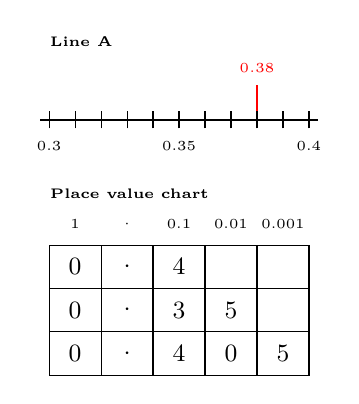
\begin{tikzpicture}[scale=1.1]

% --- Line A: 0.3 to 0.4 in hundredths ---
\node[font=\tiny\bfseries, anchor=west] at (-0.1,3.5) {Line A};
\draw[thick] (-0.1,2.6) -- (3.1,2.6);
\foreach \x in {0,0.3,0.6,0.9,1.2,1.5,1.8,2.1,2.4,2.7,3}
  \draw (\x,2.5) -- (\x,2.7);
\foreach \x/\lab in {0/0.3,1.5/0.35,3/0.4} \node[font=\tiny] at (\x,2.3) {\lab};
% --- Q5 answer: 0.38 marked ---
\draw[ans] (2.4,2.7) -- (2.4,3.0);
\node[anslab] at (2.4,3.2) {$0.38$};

% --- Place value chart: 0.4, 0.35, 0.405 ---
\node[font=\tiny\bfseries, anchor=west] at (-0.1,1.75) {Place value chart};
\foreach \i/\head in {0/1,1/{$\cdot$},2/0.1,3/0.01,4/0.001}
  \node[font=\tiny] at ({0.6*\i+0.3},1.4) {\head};
\foreach \j in {0,1,2} {
  \foreach \i in {0,1,2,3,4}
    \draw ({0.6*\i},{-0.5*\j+1.15}) rectangle ({0.6*\i+0.6},{-0.5*\j+0.65});
}
% row 1: 0.4
\foreach \i/\d in {0/0,1/{$\cdot$},2/4} \node[font=\small] at ({0.6*\i+0.3},0.9) {\d};
% row 2: 0.35
\foreach \i/\d in {0/0,1/{$\cdot$},2/3,3/5} \node[font=\small] at ({0.6*\i+0.3},0.4) {\d};
% row 3: 0.405
\foreach \i/\d in {0/0,1/{$\cdot$},2/4,3/0,4/5} \node[font=\small] at ({0.6*\i+0.3},-0.1) {\d};

\end{tikzpicture}
\end{center}

\column{0.72\textwidth}

\small
\begin{multicols}{2}
\begin{enumerate}\qtight

  \item Fill in $<$ or $>$: $7 \mathrel{\text{\ashow{$<$}}} 12$\newline $30 \mathrel{\text{\ashow{$>$}}} 3$
  \vspace{1em}

  \item In $0.405$, what is the $4$ worth? \ashow{$4$ tenths, $0.4$}

  \item On the place value chart, which is bigger, $0.4$ or $0.35$? Why? \ashow{$0.4$: $4$ tenths is greater than $3$ tenths}

  \item Fill in $<$, $>$ or $=$ $0.4 \mathrel{\text{\ashow{$=$}}} 0.40$, $0.6 \mathrel{\text{\ashow{$>$}}} 0.06$

\vspace{0.5em}

  \item Mark $0.38$ on Line A. Is it nearer $0.3$ or $0.4$? \ashow{nearer $0.4$}

  \columnbreak

  \item Order, smallest first: $0.5$, $0.45$, $0.405$, $0.54$ \ashow{$0.405$, $0.45$, $0.5$, $0.54$}

  \vspace{0.2em}

  \item True or false: more digits \emph{after} the decimal point means a bigger number? Give an example/counter-example. \ashow{False: $0.9>0.1234$}

  \vspace{0.2em}

  \item Alfie says $0.45>0.5$ as $45>5$. Explain his mistake, then write a decimal between $0.4$ and $0.405$. \ashow{$0.5$ has $5$ tenths; e.g.\ $0.402$}

\end{enumerate}
\end{multicols}

\end{columns}

\end{frame}

\begin{frame}{Worked Solution: Retrieve and Connect 2, Question 1}
\hypertarget{work-st2}{}
\textbf{Question:} Fill in $<$ or $>$: $7 \mathrel{\text{}} 12$; $30 \mathrel{\text{}} 3$.
\awork{Solution: \(7<12\) because 7 is less than 12. \(30>3\) because 30 is greater than 3.}
\end{frame}

\begin{frame}{Worked Solution: Retrieve and Connect 2, Question 2}
\textbf{Question:} In $0.405$, what is the $4$ worth?
\awork{Solution: The digit \(4\) is in the tenths place, so it is worth \(4\) tenths, i.e.\ \(0.4\).}
\end{frame}

\begin{frame}{Worked Solution: Retrieve and Connect 2, Question 3}
\textbf{Question:} On the place value chart, which is bigger, $0.4$ or $0.35$? Why?
\awork{Solution: \(0.4\) is bigger. Write \(0.4=0.40\), which is 4 tenths and 0 hundredths. \(0.35\) is 3 tenths and 5 hundredths. Comparing tenths, 4 tenths is greater than 3 tenths, so \(0.4>0.35\).}
\end{frame}

\begin{frame}{Worked Solution: Retrieve and Connect 2, Question 4}
\textbf{Question:} Fill in $<$, $>$ or $=$: $0.4 \mathrel{\text{}} 0.40$, $0.6 \mathrel{\text{}} 0.06$.
\awork{Solution: \(0.4=0.40\) because the trailing zero does not change the value. \(0.6=0.60\), which is 60 hundredths, while \(0.06\) is 6 hundredths; so \(0.6>0.06\).}
\end{frame}

\begin{frame}{Worked Solution: Retrieve and Connect 2, Question 5}
\textbf{Question:} Mark $0.38$ on Line A. Is it nearer $0.3$ or $0.4$?
\awork{Solution: \(0.38\) is 8 hundredths from \(0.3\) and 2 hundredths from \(0.4\). Since 2 is less than 8, \(0.38\) is nearer \(0.4\). On the line it lies two small ticks before \(0.4\).}
\end{frame}

\begin{frame}{Worked Solution: Retrieve and Connect 2, Question 6}
\textbf{Question:} Order, smallest first: $0.5$, $0.45$, $0.405$, $0.54$.
\awork{Solution: Write all to three decimal places: \(0.500, 0.450, 0.405, 0.540\). Comparing these gives \(0.405 < 0.450 < 0.500 < 0.540\). So the order is \(0.405, 0.45, 0.5, 0.54\).}
\end{frame}

\begin{frame}{Worked Solution: Retrieve and Connect 2, Question 7}
\textbf{Question:} True or false: more digits \emph{after} the decimal point means a bigger number? Give an example/counter-example.
\awork{Solution: False. The value depends on place value, not the number of digits. For example, \(0.9>0.1234\): \(0.9\) is 9 tenths, while \(0.1234\) is only slightly more than 1 tenth.}
\end{frame}

\begin{frame}{Worked Solution: Retrieve and Connect 2, Question 8}
\textbf{Question:} Alfie says $0.45>0.5$ as $45>5$. Explain his mistake, then write a decimal between $0.4$ and $0.405$.
\awork{Solution: Alfie compared the digits \(45\) and \(5\) as whole numbers, ignoring their place values. In \(0.5\), the 5 is in the tenths place, so \(0.5=0.50\), which is greater than \(0.45\) (4 tenths and 5 hundredths). A decimal between \(0.4\) and \(0.405\) is, for example, \(0.402\).}
\end{frame}

%------------------------------------------------
% STARTER 3: Negative Numbers
%------------------------------------------------
\begin{frame}{Retrieve and Connect: Ordering Negative Numbers}
\hypertarget{q-st3}{}

\vspace{-2.5em}

\begin{columns}[T]

\column{0.30\textwidth}
\begin{center}
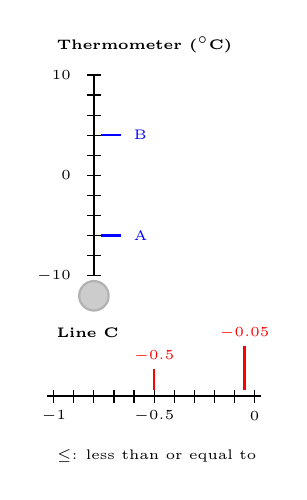
\begin{tikzpicture}[scale=0.85]

% --- Thermometer: -10 to 10, one tick every 2 degrees, only -10/0/10 labelled ---
\node[font=\tiny\bfseries, anchor=west] at (-0.1,3.45) {Thermometer ($^\circ$C)};
\draw[thick] (0.6,0) -- (0.6,3);
\foreach \y in {0,0.3,0.6,0.9,1.2,1.5,1.8,2.1,2.4,2.7,3}
  \draw (0.5,\y) -- (0.7,\y);
\foreach \y/\lab in {0/{$-10$},1.5/{$0$},3/{$10$}}
  \node[font=\tiny, anchor=east] at (0.4,\y) {\lab};
\fill[gray!40] (0.6,-0.3) circle (0.22);
\draw[gray!60, thick] (0.6,-0.3) circle (0.22);
% Given readings: A at -6, B at 4 (both sit exactly on a tick)
\draw[blue, thick] (0.7,0.6) -- (1.0,0.6);
\node[blue, font=\tiny, anchor=west] at (1.05,0.6) {A};
\draw[blue, thick] (0.7,2.1) -- (1.0,2.1);
\node[blue, font=\tiny, anchor=west] at (1.05,2.1) {B};

% --- Line C: -1 to 0 in tenths ---
\node[font=\tiny\bfseries, anchor=west] at (-0.1,-0.85) {Line C};
\draw[thick] (-0.1,-1.8) -- (3.1,-1.8);
\foreach \x in {0,0.3,0.6,0.9,1.2,1.5,1.8,2.1,2.4,2.7,3}
  \draw (\x,-1.9) -- (\x,-1.7);
\foreach \x/\lab in {0/{$-1$},1.5/{$-0.5$},3/{$0$}} \node[font=\tiny] at (\x,-2.1) {\lab};
% Reminder for the challenge question, which is the deck's only use of a weak inequality
\node[font=\tiny, anchor=west] at (-0.1,-2.7) {$\leq$: less than or equal to};
% --- Q5 answers: -0.5 and -0.05 marked on Line C, at different heights ---
\draw[ans] (1.5,-1.7) -- (1.5,-1.4);
\node[anslab] at (1.5,-1.2) {$-0.5$};
\draw[ans] (2.85,-1.7) -- (2.85,-1.05);
\node[anslab] at (2.85,-0.85) {$-0.05$};

\end{tikzpicture}
\end{center}

\column{0.70\textwidth}

\small
\begin{multicols}{2}
\begin{enumerate}\qtight

  \item Which is colder, $4\,^\circ$C or $-4\,^\circ$C? \ashow{$-4\,^\circ$C}

  \item What is each mark on the thermometer worth? Write the temperatures at A and B. \ashow{$2\,^\circ$C per mark; A $=-6$, B $=4$}

  \item Which is colder, $-3$ or $-8$? Fill in: $-3 \mathrel{\text{\ashowq{$>$}}} -8$ \ashow{($-8$ is colder)}

  \item Order, smallest first: $-2$, $5$, $-7$, $0$, $-1$ \ashow{($-7,-2,-1,0,5$)}

  \columnbreak

  \item Mark $-0.5$ and $-0.05$ on Line C. Which is larger? \ashow{$-0.05$}

  \item Fill in $<$ or $>$: $-4.5 \mathrel{\text{\ashowq{$<$}}} -4.05$, $-0.3 \mathrel{\text{\ashowq{$<$}}} 0.03$

  \item (Extension) Order, smallest first: $-0.08$, $0.7$, $-0.8$, $-0.75$ \ashow{($-0.8$, $-0.75$, $-0.08$, $0.7$)}

  \item (Challenge) List the integers $n$: $-3\leq n<2$. Write a number between $-0.5$ and $-0.4$. \ashow{$-3,-2,-1,0,1$; e.g.\ $-0.45$}

\end{enumerate}
\end{multicols}

\end{columns}

\end{frame}

\begin{frame}{Worked Solution: Retrieve and Connect 3, Question 1}
\hypertarget{work-st3}{}
\textbf{Question:} Which is colder, $4\,^\circ$C or $-4\,^\circ$C?
\awork{Solution: \(-4\,^\circ\)C is colder. Negative temperatures are below zero, so \(-4\,^\circ\)C is 4 degrees below freezing, whereas \(4\,^\circ\)C is 4 degrees above freezing.}
\end{frame}

\begin{frame}{Worked Solution: Retrieve and Connect 3, Question 2}
\textbf{Question:} What is each mark on the thermometer worth? Write the temperatures at A and B.
\awork{Solution: The thermometer goes from \(-10\) to \(10\), a total of 20 degrees, with 10 equal intervals. So each mark is \(20\div10=2\,^\circ\)C. Point A is 2 marks above \(-10\): \(-10+2\times2=-6\,^\circ\)C. Point B is 2 marks above 0: \(0+2\times2=4\,^\circ\)C.}
\end{frame}

\begin{frame}{Worked Solution: Retrieve and Connect 3, Question 3}
\textbf{Question:} Which is colder, $-3$ or $-8$? Fill in: $-3 \mathrel{\text{}} -8$.
\awork{Solution: \(-8\) is colder because it is further below zero. On a number line, \(-8\) is to the left of \(-3\), so \(-3>-8\). The correct symbol is \(>\).}
\end{frame}

\begin{frame}{Worked Solution: Retrieve and Connect 3, Question 4}
\textbf{Question:} Order, smallest first: $-2$, $5$, $-7$, $0$, $-1$.
\awork{Solution: On a number line, more negative numbers are smaller. The negative numbers in order are \(-7, -2, -1\). Then come 0 and 5. So the order is \(-7, -2, -1, 0, 5\).}
\end{frame}

\begin{frame}{Worked Solution: Retrieve and Connect 3, Question 5}
\textbf{Question:} Mark $-0.5$ and $-0.05$ on Line C. Which is larger?
\awork{Solution: Line C goes from \(-1\) to \(0\) in tenths. \(-0.5\) is halfway between \(-1\) and \(0\). \(-0.05\) is very close to \(0\), just 5 hundredths to the left of \(0\). Since \(-0.05\) is closer to \(0\), it is larger: \(-0.05>-0.5\).}
\end{frame}

\begin{frame}{Worked Solution: Retrieve and Connect 3, Question 6}
\textbf{Question:} Fill in $<$ or $>$: $-4.5 \mathrel{\text{}} -4.05$, $-0.3 \mathrel{\text{}} 0.03$.
\awork{Solution: \(-4.5\) is more negative than \(-4.05\), so \(-4.5<-4.05\). Any negative number is less than any positive number, so \(-0.3<0.03\).}
\end{frame}

\begin{frame}{Worked Solution: Retrieve and Connect 3, Question 7}
\textbf{Question:} (Extension) Order, smallest first: $-0.08$, $0.7$, $-0.8$, $-0.75$.
\awork{Solution: First order the negative numbers: \(-0.8<-0.75<-0.08\). The positive number \(0.7\) is larger than all of them. So the order is \(-0.8, -0.75, -0.08, 0.7\).}
\end{frame}

\begin{frame}{Worked Solution: Retrieve and Connect 3, Question 8}
\textbf{Question:} (Challenge) List the integers $n$: $-3\leq n<2$. Write a number between $-0.5$ and $-0.4$.
\awork{Solution: The integers satisfying \(-3\le n<2\) are \(-3, -2, -1, 0, 1\). (The value 2 is not included because the inequality is strict.) A number between \(-0.5\) and \(-0.4\) is, for example, \(-0.45\).}
\end{frame}

%------------------------------------------------
% STARTER 4: Rounding Integers
%------------------------------------------------
\begin{frame}{Retrieve and Connect: Rounding Integers}
\hypertarget{q-st4}{}

\vspace{-2.5em}

\begin{columns}[T]

\column{0.30\textwidth}
\begin{center}
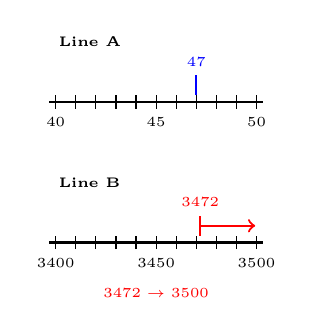
\begin{tikzpicture}[scale=0.85]

% --- Line A: 40 to 50, ticks every 1 ---
\node[font=\tiny\bfseries, anchor=west] at (-0.1,3.5) {Line A};
\draw[thick] (-0.1,2.6) -- (3.1,2.6);
\foreach \x in {0,0.3,0.6,0.9,1.2,1.5,1.8,2.1,2.4,2.7,3}
  \draw (\x,2.5) -- (\x,2.7);
\foreach \x/\lab in {0/40,1.5/45,3/50} \node[font=\tiny] at (\x,2.3) {\lab};
% Given point: 47
\draw[blue, thick] (2.1,2.7) -- (2.1,3.0);
\node[blue, font=\tiny] at (2.1,3.2) {$47$};

% --- Line B: 3400 to 3500, ticks every 10 ---
\node[font=\tiny\bfseries, anchor=west] at (-0.1,1.4) {Line B};
\draw[thick] (-0.1,0.5) -- (3.1,0.5);
\foreach \x in {0,0.3,0.6,0.9,1.2,1.5,1.8,2.1,2.4,2.7,3}
  \draw (\x,0.4) -- (\x,0.6);
\foreach \x/\lab in {0/3400,1.5/3450,3/3500} \node[font=\tiny] at (\x,0.2) {\lab};
% --- Q4 answers: 3472 marked, with an arrow to the nearer end ---
\draw[ans] (2.16,0.6) -- (2.16,0.9);
\node[anslab] at (2.16,1.1) {$3472$};
\draw[ans, ->] (2.16,0.75) -- (2.98,0.75);
\node[anslab] at (1.5,-0.25) {$3472 \to 3500$};

\end{tikzpicture}
\end{center}

\column{0.70\textwidth}

\small
\begin{multicols}{2}
\begin{enumerate}\qtight

  \item Fill in $<$ or $>$: $-6 \mathrel{\text{\ashowq{$<$}}} -2$

  \item Line A: is $47$ nearer $40$ or $50$? Round it to the nearest $10$. \ashow{nearer $50$, so $50$}

  \item Round to the nearest $10$: $32$, $85$ \ashow{($30$ and $90$)}

  \item Mark $3472$ on Line B, then round it to the nearest $100$.

  \item Round $3472$ to the nearest $10$; to the nearest $1000$. \ashow{$3470$ and $3000$}

  \columnbreak

  \item Round $4950$ to the nearest $100$. \ashow{$5000$}

  \item Zoe rounds $8449$ to the nearest $100$: $8449\to 8450\to 8500$. What is her mistake? \ashow{Rounded twice: only the tens digit $4$ counts, so $8400$}

  \item A number rounded to the nearest $10$ is $250$. What is the smallest it could be? The largest? \ashow{$245$ and $254$}

\end{enumerate}
\end{multicols}

\end{columns}

\end{frame}

\begin{frame}{Worked Solution: Retrieve and Connect 4, Question 1}
\hypertarget{work-st4}{}
\textbf{Question:} Fill in $<$ or $>$: $-6 \mathrel{\text{}} -2$.
\awork{Solution: \(-6\) is to the left of \(-2\) on a number line, so \(-6<-2\). The correct symbol is \(<\).}
\end{frame}

\begin{frame}{Worked Solution: Retrieve and Connect 4, Question 2}
\textbf{Question:} Line A: is $47$ nearer $40$ or $50$? Round it to the nearest $10$.
\awork{Solution: \(47\) is 7 away from \(40\) and 3 away from \(50\). Since 3 is less than 7, it is nearer \(50\). Rounding to the nearest 10 gives \(50\).}
\end{frame}

\begin{frame}{Worked Solution: Retrieve and Connect 4, Question 3}
\textbf{Question:} Round to the nearest $10$: $32$, $85$.
\awork{Solution: For \(32\), the units digit is 2, which is less than 5, so round down to \(30\). For \(85\), the units digit is 5, so round up to \(90\).}
\end{frame}

\begin{frame}{Worked Solution: Retrieve and Connect 4, Question 4}
\textbf{Question:} Mark $3472$ on Line B, then round it to the nearest $100$.
\awork{Solution: Line B goes from 3400 to 3500 in steps of 10. \(3472\) is between \(3470\) and \(3480\). To round to the nearest 100, look at the tens digit, which is 7. Since \(7\ge5\), round up to \(3500\). It is also nearer 3500 than 3400.}
\end{frame}

\begin{frame}{Worked Solution: Retrieve and Connect 4, Question 5}
\textbf{Question:} Round $3472$ to the nearest $10$; to the nearest $1000$.
\awork{Solution: To the nearest 10: look at the units digit 2, so \(3472\to3470\). To the nearest 1000: look at the hundreds digit 4. Since \(4<5\), round down to \(3000\). (It is 472 from 3000 and 528 from 4000.)}
\end{frame}

\begin{frame}{Worked Solution: Retrieve and Connect 4, Question 6}
\textbf{Question:} Round $4950$ to the nearest $100$.
\awork{Solution: To round to the nearest 100, look at the tens digit, which is 5. Since \(5\ge5\), round up. So \(4950\to5000\).}
\end{frame}

\begin{frame}{Worked Solution: Retrieve and Connect 4, Question 7}
\textbf{Question:} Zoe rounds $8449$ to the nearest $100$: $8449\to 8450\to 8500$. What is her mistake?
\awork{Solution: Zoe rounded twice. To round directly to the nearest 100, look only at the tens digit. In \(8449\), the tens digit is 4, and \(4<5\), so \(8449\) rounds down to \(8400\). The first rounding to \(8450\) should not be used again.}
\end{frame}

\begin{frame}{Worked Solution: Retrieve and Connect 4, Question 8}
\textbf{Question:} A number rounded to the nearest $10$ is $250$. What is the smallest it could be? The largest?
\awork{Solution: For a whole number, the values that round to 250 are those from 245 up to 254. \(245\) rounds up to 250, and \(254\) rounds down to 250. So the smallest is \(245\) and the largest is \(254\).}
\end{frame}

%------------------------------------------------
% STARTER 5: Rounding Decimals, Recurring and Irrational
%------------------------------------------------
\begin{frame}{Retrieve and Connect: Rounding Decimals \& Never-Ending Decimals}
\hypertarget{q-st5}{}

\vspace{-2.5em}

\begin{columns}[T]

\column{0.30\textwidth}
\begin{center}
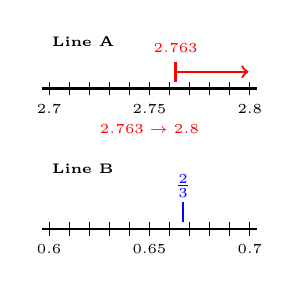
\begin{tikzpicture}[scale=0.85]

% --- Line A: 2.7 to 2.8 in hundredths ---
% Heading sits at 3.3 rather than 3.5: this frame's title is two lines' worth of
% width and the diagram column otherwise crowds it.
\node[font=\tiny\bfseries, anchor=west] at (-0.1,3.3) {Line A};
\draw[thick] (-0.1,2.6) -- (3.1,2.6);
\foreach \x in {0,0.3,0.6,0.9,1.2,1.5,1.8,2.1,2.4,2.7,3}
  \draw (\x,2.5) -- (\x,2.7);
\foreach \x/\lab in {0/2.7,1.5/2.75,3/2.8} \node[font=\tiny] at (\x,2.3) {\lab};
% (the Line A heading sits low here, to keep clear of the frame title)
% --- Q3 answers: 2.763 marked, with an arrow to the nearer end ---
\draw[ans] (1.89,2.7) -- (1.89,3.0);
\node[anslab] at (1.89,3.2) {$2.763$};
\draw[ans, ->] (1.89,2.85) -- (2.98,2.85);
\node[anslab] at (1.5,2.0) {$2.763 \to 2.8$};

% --- Line B: 0.6 to 0.7 in hundredths, with 2/3 shown ---
\node[font=\tiny\bfseries, anchor=west] at (-0.1,1.4) {Line B};
\draw[thick] (-0.1,0.5) -- (3.1,0.5);
\foreach \x in {0,0.3,0.6,0.9,1.2,1.5,1.8,2.1,2.4,2.7,3}
  \draw (\x,0.4) -- (\x,0.6);
\foreach \x/\lab in {0/0.6,1.5/0.65,3/0.7} \node[font=\tiny] at (\x,0.2) {\lab};
% Given point: 2/3 = 0.6666...
\draw[blue, thick] (2.0,0.6) -- (2.0,0.9);
\node[blue, font=\scriptsize] at (2.0,1.15) {$\tfrac{2}{3}$};

\end{tikzpicture}

\vspace{0.4em}
{\scriptsize
\begin{tabular}{@{}l@{}}
\textbf{Never-ending decimals} \\[0.15em]
$\frac{2}{3} = 0.6666\ldots = 0.\dot{6}$ \\
$\frac{1}{7} = 0.142857142857\ldots$ \\
$\pi = 3.14159265\ldots$ \\
$\sqrt{2} = 1.41421356\ldots$ \\
$0.1010010001\ldots$
\end{tabular}}
\end{center}

\column{0.70\textwidth}

\small
\begin{multicols}{2}
\begin{enumerate}\qtight

  \item Round $4738$ to the nearest $100$. \ashow{$4700$}

  \item Round to the nearest whole number: $4.6$, $12.348$ \ashow{($5$ and $12$)}

  \item Mark $2.763$ on Line A. Round it to $1$ decimal place (d.p.).

  \item Round to $1$ d.p.: $4.62$, $0.95$. Why is $0.95$ not $1$? \ashow{$4.6$, $1.0$ --- $1$ d.p.\ needs one decimal digit}

  \item Round $12.348$ to $2$ d.p., then to $1$ d.p. Why not $12.4$? \ashow{$12.35$, $12.3$ --- never round twice}

  \columnbreak

  \item Line B shows $\frac{2}{3}=0.\dot{6}$. Round it to $1$ d.p.\ and $2$ d.p. \ashow{$0.7$ and $0.67$}

  \item (Extension) Write $\frac{1}{3}$ in dot notation, then round $\frac{1}{7}$ to $3$ d.p. \ashow{$0.\dot{3}$ and $0.143$}

  \item (Challenge) Which listed decimals never settle into a repeating block? Can one still be a fraction? \ashow{$\pi$, $\sqrt{2}$, $0.101001\ldots$; yes: $0.\dot{3}=\frac13$}

\end{enumerate}
\end{multicols}

\end{columns}

\end{frame}

\begin{frame}{Worked Solution: Retrieve and Connect 5, Question 1}
\hypertarget{work-st5}{}
\textbf{Question:} Round $4738$ to the nearest $100$.
\awork{Solution: To round to the nearest 100, look at the tens digit. In \(4738\), the tens digit is 3. Since \(3<5\), round down to \(4700\).}
\end{frame}

\begin{frame}{Worked Solution: Retrieve and Connect 5, Question 2}
\textbf{Question:} Round to the nearest whole number: $4.6$, $12.348$.
\awork{Solution: For \(4.6\), the tenths digit is 6, so round up to \(5\). For \(12.348\), the tenths digit is 3, so round down to \(12\).}
\end{frame}

\begin{frame}{Worked Solution: Retrieve and Connect 5, Question 3}
\textbf{Question:} Mark $2.763$ on Line A. Round it to $1$ decimal place (d.p.).
\awork{Solution: Line A goes from 2.7 to 2.8 in hundredths. \(2.763\) lies between \(2.76\) and \(2.77\), closer to \(2.76\). To round to 1 d.p., look at the hundredths digit: in \(2.763\), the tenths digit is 7 and the hundredths digit is 6. Since \(6\ge5\), round up to \(2.8\).}
\end{frame}

\begin{frame}{Worked Solution: Retrieve and Connect 5, Question 4}
\textbf{Question:} Round to $1$ d.p.: $4.62$, $0.95$. Why is $0.95$ not $1$?
\awork{Solution: \(4.62\) to 1 d.p.: the hundredths digit is 2, so \(4.62\to4.6\). \(0.95\) to 1 d.p.: the hundredths digit is 5, so round up; \(0.9\) becomes \(1.0\). It is written as \(1.0\) rather than \(1\) because 1 d.p.\ requires exactly one digit after the decimal point.}
\end{frame}

\begin{frame}{Worked Solution: Retrieve and Connect 5, Question 5}
\textbf{Question:} Round $12.348$ to $2$ d.p., then to $1$ d.p. Why not $12.4$?
\awork{Solution: To 2 d.p., look at the third decimal digit in \(12.348\), which is 8. So \(12.348\to12.35\). To 1 d.p., round the original number directly: the hundredths digit in \(12.348\) is 4, so \(12.348\to12.3\). It is not \(12.4\) because you should not round twice (\(12.348\to12.35\to12.4\) is double rounding).}
\end{frame}

\begin{frame}{Worked Solution: Retrieve and Connect 5, Question 6}
\textbf{Question:} Line B shows $\frac{2}{3}=0.\dot{6}$. Round it to $1$ d.p.\ and $2$ d.p.
\awork{Solution: \(0.\dot{6}=0.6666\ldots\). To 1 d.p., look at the hundredths digit 6, so round up: \(0.7\). To 2 d.p., look at the third decimal digit 6, so round up: \(0.67\).}
\end{frame}

\begin{frame}{Worked Solution: Retrieve and Connect 5, Question 7}
\textbf{Question:} (Extension) Write $\frac{1}{3}$ in dot notation, then round $\frac{1}{7}$ to $3$ d.p.
\awork{Solution: \(\frac13=0.3333\ldots=0.\dot{3}\). \(\frac17=0.142857142857\ldots\). To 3 d.p., look at the fourth decimal digit, which is 8, so round up: \(0.143\).}
\end{frame}

\begin{frame}{Worked Solution: Retrieve and Connect 5, Question 8}
\textbf{Question:} (Challenge) Which listed decimals never settle into a repeating block? Can one still be a fraction?
\awork{Solution: The decimals that never settle into a repeating block are \(\pi\), \(\sqrt{2}\), and \(0.1010010001\ldots\). These are non-repeating, non-terminating. A never-ending decimal can still be a fraction if it repeats, for example \(0.\dot{3}=\frac13\). The non-repeating ones are irrational and cannot be written as fractions.}
\end{frame}

\end{document}